% Options for packages loaded elsewhere
\PassOptionsToPackage{unicode}{hyperref}
\PassOptionsToPackage{hyphens}{url}
\PassOptionsToPackage{dvipsnames,svgnames,x11names}{xcolor}
%
\documentclass[
  letterpaper,
  DIV=11,
  numbers=noendperiod]{scrartcl}

\usepackage{amsmath,amssymb}
\usepackage{iftex}
\ifPDFTeX
  \usepackage[T1]{fontenc}
  \usepackage[utf8]{inputenc}
  \usepackage{textcomp} % provide euro and other symbols
\else % if luatex or xetex
  \usepackage{unicode-math}
  \defaultfontfeatures{Scale=MatchLowercase}
  \defaultfontfeatures[\rmfamily]{Ligatures=TeX,Scale=1}
\fi
\usepackage{lmodern}
\ifPDFTeX\else  
    % xetex/luatex font selection
\fi
% Use upquote if available, for straight quotes in verbatim environments
\IfFileExists{upquote.sty}{\usepackage{upquote}}{}
\IfFileExists{microtype.sty}{% use microtype if available
  \usepackage[]{microtype}
  \UseMicrotypeSet[protrusion]{basicmath} % disable protrusion for tt fonts
}{}
\makeatletter
\@ifundefined{KOMAClassName}{% if non-KOMA class
  \IfFileExists{parskip.sty}{%
    \usepackage{parskip}
  }{% else
    \setlength{\parindent}{0pt}
    \setlength{\parskip}{6pt plus 2pt minus 1pt}}
}{% if KOMA class
  \KOMAoptions{parskip=half}}
\makeatother
\usepackage{xcolor}
\setlength{\emergencystretch}{3em} % prevent overfull lines
\setcounter{secnumdepth}{-\maxdimen} % remove section numbering
% Make \paragraph and \subparagraph free-standing
\ifx\paragraph\undefined\else
  \let\oldparagraph\paragraph
  \renewcommand{\paragraph}[1]{\oldparagraph{#1}\mbox{}}
\fi
\ifx\subparagraph\undefined\else
  \let\oldsubparagraph\subparagraph
  \renewcommand{\subparagraph}[1]{\oldsubparagraph{#1}\mbox{}}
\fi


\providecommand{\tightlist}{%
  \setlength{\itemsep}{0pt}\setlength{\parskip}{0pt}}\usepackage{longtable,booktabs,array}
\usepackage{calc} % for calculating minipage widths
% Correct order of tables after \paragraph or \subparagraph
\usepackage{etoolbox}
\makeatletter
\patchcmd\longtable{\par}{\if@noskipsec\mbox{}\fi\par}{}{}
\makeatother
% Allow footnotes in longtable head/foot
\IfFileExists{footnotehyper.sty}{\usepackage{footnotehyper}}{\usepackage{footnote}}
\makesavenoteenv{longtable}
\usepackage{graphicx}
\makeatletter
\def\maxwidth{\ifdim\Gin@nat@width>\linewidth\linewidth\else\Gin@nat@width\fi}
\def\maxheight{\ifdim\Gin@nat@height>\textheight\textheight\else\Gin@nat@height\fi}
\makeatother
% Scale images if necessary, so that they will not overflow the page
% margins by default, and it is still possible to overwrite the defaults
% using explicit options in \includegraphics[width, height, ...]{}
\setkeys{Gin}{width=\maxwidth,height=\maxheight,keepaspectratio}
% Set default figure placement to htbp
\makeatletter
\def\fps@figure{htbp}
\makeatother
\newlength{\cslhangindent}
\setlength{\cslhangindent}{1.5em}
\newlength{\csllabelwidth}
\setlength{\csllabelwidth}{3em}
\newlength{\cslentryspacingunit} % times entry-spacing
\setlength{\cslentryspacingunit}{\parskip}
\newenvironment{CSLReferences}[2] % #1 hanging-ident, #2 entry spacing
 {% don't indent paragraphs
  \setlength{\parindent}{0pt}
  % turn on hanging indent if param 1 is 1
  \ifodd #1
  \let\oldpar\par
  \def\par{\hangindent=\cslhangindent\oldpar}
  \fi
  % set entry spacing
  \setlength{\parskip}{#2\cslentryspacingunit}
 }%
 {}
\usepackage{calc}
\newcommand{\CSLBlock}[1]{#1\hfill\break}
\newcommand{\CSLLeftMargin}[1]{\parbox[t]{\csllabelwidth}{#1}}
\newcommand{\CSLRightInline}[1]{\parbox[t]{\linewidth - \csllabelwidth}{#1}\break}
\newcommand{\CSLIndent}[1]{\hspace{\cslhangindent}#1}

% load packages
\usepackage{geometry}
\usepackage{xcolor}
\usepackage{eso-pic}
\usepackage{fancyhdr}
\usepackage{sectsty}
\usepackage{fontspec}
\usepackage{titlesec}

%% Set page size with a wider right margin
\geometry{a4paper, total={170mm,257mm}, left=20mm, top=20mm, bottom=20mm, right=50mm}

%% Let's define some colours
\definecolor{light}{HTML}{1CABE2}
\definecolor{highlight}{HTML}{374EA2}
\definecolor{dark}{HTML}{2D2926}

%% Let's add the border on the right hand side 
\AddToShipoutPicture{% 
    \AtPageLowerLeft{% 
        \put(\LenToUnit{\dimexpr\paperwidth-3cm},0){% 
            \color{light}\rule{3cm}{\LenToUnit\paperheight}%
          }%
     }%
     % logo
    \AtPageLowerLeft{% start the bar at the bottom right of the page
        \put(\LenToUnit{\dimexpr\paperwidth-2.25cm},27.2cm){% move it to the top right
          }%
     }%
}

%% Style the page number
\fancypagestyle{mystyle}{
  \fancyhf{}
  \renewcommand\headrulewidth{0pt}
  \fancyfoot[R]{\thepage}
  \fancyfootoffset{3.5cm}
}
\setlength{\footskip}{20pt}

%% style the chapter/section fonts
\chapterfont{\color{dark}\fontsize{16}{20}\selectfont}
\sectionfont{\color{dark}\fontsize{16}{16.8}\selectfont}
\subsectionfont{\color{dark}\fontsize{14}{16.8}\selectfont}
\titleformat{\subsection}
  {\sffamily\Large\bfseries}{\thesection}{1em}{}[{\titlerule[0.8pt]}]
  
% left align title
\makeatletter
\renewcommand{\maketitle}{\bgroup\setlength{\parindent}{0pt}
\begin{flushleft}
  {\sffamily\huge\textbf{\MakeUppercase{\@title}}} \vspace{0.3cm} \newline
  {\Large {\@subtitle}} \newline
  \@author
\end{flushleft}\egroup
}
\makeatother

%% Use some custom fonts
\setsansfont{Ubuntu}[
    Path=_extensions/nrennie/PrettyPDF/Ubuntu/,
    Scale=0.9,
    Extension = .ttf,
    UprightFont=*-Regular,
    BoldFont=*-Bold,
    ItalicFont=*-Italic,
    ]

\setmainfont{Ubuntu}[
    Path=_extensions/nrennie/PrettyPDF/Ubuntu/,
    Scale=0.9,
    Extension = .ttf,
    UprightFont=*-Regular,
    BoldFont=*-Bold,
    ItalicFont=*-Italic,
    ]
\KOMAoption{captions}{tableheading}
\makeatletter
\makeatother
\makeatletter
\makeatother
\makeatletter
\@ifpackageloaded{caption}{}{\usepackage{caption}}
\AtBeginDocument{%
\ifdefined\contentsname
  \renewcommand*\contentsname{Table of contents}
\else
  \newcommand\contentsname{Table of contents}
\fi
\ifdefined\listfigurename
  \renewcommand*\listfigurename{List of Figures}
\else
  \newcommand\listfigurename{List of Figures}
\fi
\ifdefined\listtablename
  \renewcommand*\listtablename{List of Tables}
\else
  \newcommand\listtablename{List of Tables}
\fi
\ifdefined\figurename
  \renewcommand*\figurename{Figure}
\else
  \newcommand\figurename{Figure}
\fi
\ifdefined\tablename
  \renewcommand*\tablename{Table}
\else
  \newcommand\tablename{Table}
\fi
}
\@ifpackageloaded{float}{}{\usepackage{float}}
\floatstyle{ruled}
\@ifundefined{c@chapter}{\newfloat{codelisting}{h}{lop}}{\newfloat{codelisting}{h}{lop}[chapter]}
\floatname{codelisting}{Listing}
\newcommand*\listoflistings{\listof{codelisting}{List of Listings}}
\makeatother
\makeatletter
\@ifpackageloaded{caption}{}{\usepackage{caption}}
\@ifpackageloaded{subcaption}{}{\usepackage{subcaption}}
\makeatother
\makeatletter
\@ifpackageloaded{tcolorbox}{}{\usepackage[skins,breakable]{tcolorbox}}
\makeatother
\makeatletter
\@ifundefined{shadecolor}{\definecolor{shadecolor}{rgb}{.97, .97, .97}}
\makeatother
\makeatletter
\@ifundefined{codebgcolor}{\definecolor{codebgcolor}{named}{light}}
\makeatother
\makeatletter
\makeatother
\ifLuaTeX
  \usepackage{selnolig}  % disable illegal ligatures
\fi
\IfFileExists{bookmark.sty}{\usepackage{bookmark}}{\usepackage{hyperref}}
\IfFileExists{xurl.sty}{\usepackage{xurl}}{} % add URL line breaks if available
\urlstyle{same} % disable monospaced font for URLs
\hypersetup{
  pdftitle={Interesting and Noteworthy Findings},
  colorlinks=true,
  linkcolor={highlight},
  filecolor={Maroon},
  citecolor={Blue},
  urlcolor={highlight},
  pdfcreator={LaTeX via pandoc}}

\title{Interesting and Noteworthy Findings}
\usepackage{etoolbox}
\makeatletter
\providecommand{\subtitle}[1]{% add subtitle to \maketitle
  \apptocmd{\@title}{\par {\large #1 \par}}{}{}
}
\makeatother
\subtitle{Implications For The Cross Cultural Study Of Parenting And
Child Development from MICS Data}
\author{}
\date{2023-12-06}

\begin{document}
\maketitle
\pagestyle{mystyle}

\ifdefined\Shaded\renewenvironment{Shaded}{\begin{tcolorbox}[colback={codebgcolor}, breakable, enhanced, frame hidden, borderline west={3pt}{0pt}{shadecolor}, boxrule=0pt, sharp corners]}{\end{tcolorbox}}\fi

\begin{figure}[H]

{\centering 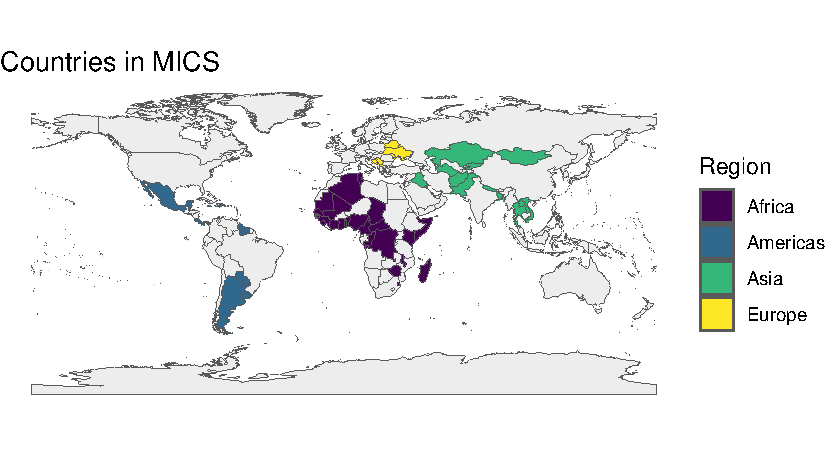
\includegraphics{MICS-infographic_files/figure-pdf/fig-MICS-1.pdf}

}

\caption{\label{fig-MICS}Countries in MICS}

\end{figure}

\hypertarget{spanking-hurts-children}{%
\section{Spanking Hurts Children}\label{spanking-hurts-children}}

Spanking is associated with decreased child socio-emotional development
\& increased child aggression.

\hypertarget{insults-contribute-to-harm}{%
\section{Insults Contribute to Harm}\label{insults-contribute-to-harm}}

Name-calling \& psychological aggression may have effects that are as
harmful as those of physical punishment.

\hypertarget{physical-and-psychological-punishment-slow-child-development}{%
\section{Physical and Psychological Punishment Slow Child
Development}\label{physical-and-psychological-punishment-slow-child-development}}

Harsh punishment is consistently associated with decreased child
socio-emotional development \& more child aggression.

\hypertarget{eliminating-spanking-reduces-abuse}{%
\section{Eliminating Spanking Reduces
Abuse}\label{eliminating-spanking-reduces-abuse}}

Simulations with MICS data suggest that eliminating spanking would
result in a large reduction in global rates of physical child abuse.

\hypertarget{use-positive-discipline}{%
\section{Use Positive Discipline!}\label{use-positive-discipline}}

Positive discipline--in the form of verbal reasoning--is associated with
improved child well-being across MICS countries.

\hypertarget{positive-discipline-benefits-children.}{%
\section{Positive discipline benefits
children.}\label{positive-discipline-benefits-children.}}

\hypertarget{references}{%
\section*{References}\label{references}}
\addcontentsline{toc}{section}{References}

\hypertarget{refs}{}
\begin{CSLReferences}{1}{0}
\leavevmode\vadjust pre{\hypertarget{ref-Grogan-Kaylor2021}{}}%
Grogan-Kaylor, Andrew, Berenice Castillo, Garrett T Pace, Kaitlin P
Ward, Julie Ma, Shawna J Lee, and Heather Knauer. 2021. {``{Global
perspectives on physical and nonphysical discipline: A Bayesian
multilevel analysis}.''} \emph{International Journal of Behavioral
Development}, January. \url{https://doi.org/10.1177/0165025420981642}.

\leavevmode\vadjust pre{\hypertarget{ref-Ma2022}{}}%
Ma, Julie, Andrew C. Grogan-Kaylor, Garrett T. Pace, Kaitlin P. Ward,
and Shawna J. Lee. 2022. {``{The association between spanking and
physical abuse of young children in 56 low- and middle-income
countries}.''} \emph{Child Abuse \& Neglect} 129 (July): 105662.
\url{https://doi.org/10.1016/j.chiabu.2022.105662}.

\leavevmode\vadjust pre{\hypertarget{ref-Pace2019}{}}%
Pace, Garrett T., Shawna J. Lee, and Andrew Grogan-Kaylor. 2019.
{``{Spanking and young children's socioemotional development in low- and
middle-income countries}.''} \emph{Child Abuse and Neglect} 88: 84--95.
\url{https://doi.org/10.1016/j.chiabu.2018.11.003}.

\leavevmode\vadjust pre{\hypertarget{ref-WardA}{}}%
Ward, Kaitlin P., Andrew C. Grogan-Kaylor, Garrett T. Pace, Jorge
Cuartas, and Shawna J. Lee. 2021a. {``{A Multilevel Ecological Analysis
of the Predictors of Spanking Across 65 Countries}.''} \emph{BMJ Open}
11 (e046075). \url{https://doi.org/10.1136/bmjopen-2020-046075}.

\leavevmode\vadjust pre{\hypertarget{ref-ward_grogan-kaylor_ma_pace_lee_2021}{}}%
Ward, Kaitlin P, Andrew Grogan-Kaylor, Julie Ma, Garrett T Pace, and
Shawna J Lee. 2021b. {``Associations Between 11 Parental Discipline
Behaviors and Child Outcomes Across 60 Countries.''} PsyArXiv.
\url{https://doi.org/10.31234/osf.io/f5t8x}.

\leavevmode\vadjust pre{\hypertarget{ref-WardC}{}}%
Ward, Kaitlin P., Shawna J. Lee, Andrew C. Grogan-Kaylor, Julie Ma, and
Garrett T. Pace. 2022. {``{Patterns of Caregiver Aggressive and
Nonaggressive Discipline Toward Young Children in Low- and Middle-Income
Countries: A Latent Class Approach}.''} \emph{Child Abuse \& Neglect}
128. https://doi.org/\url{https://doi.org/10.1016/j.chiabu.2022.105606}.

\end{CSLReferences}



\end{document}
